\section{Runge-Kutta Tracking}
Next we use the following subsections to describe in detail the Runge-Kutta
(RK) methods used to track the blowup point both forwards and backwards in
time.  Starting with the transport equation of a point, namely
\begin{equation}
    \dv{\mathbf{x}}{t}  = \mathbf{u}
\end{equation}
where $\mathbf{x}$ is the coordinate vector ($\mathbf{x} = x_{i} = \left(x_{1},
x_{2}, x_{3} \right)$) and $\mathbf{u}$ is the velocity at point $i$.  
Thus, we get the following three differential equations for each coordinate
point,
\begin{subequations}
    \begin{equation}
        \dv{x_{1}}{t} = u_{1}
        \label{eq:x1-transport}
    \end{equation}
    \begin{equation}
        \dv{x_{2}}{t} = u_{2}
        \label{eq:x2-transport}
    \end{equation}
    \begin{equation}
        \dv{x_{3}}{t} = u_{3}
        \label{eq:x3-transport}
    \end{equation}
\end{subequations}
Equations~(\ref{eq:x1-transport}-\ref{eq:x2-transport}) provide the basic
coordinate vector transport used in both the forward and backward tracking
schemes.

\subsection{Forwards Tracking}
For the forward tracking a fully explicit fourth order RK time integration
scheme was used in order to remain consistent with the ALES pseudo spectral
code. We start by converting the continuous coordinate transport equations
given in Eqs.~(\ref{eq:x1-transport}-\ref{eq:x3-transport}) to discrete
equations, we will however restrict the derivation to a single point
$x=x_{1}$ even though the subsequent derivation is applied to all three
coordinate points,  
\begin{equation}
    \dv{x_{1}}{t} =  u_{1}(\mathbf{x},t) \approx f(x_{i},t^{n})
    \label{eq:x1-discrete-space}
\end{equation}                               
where $n$ is the time step, $i$ is the spatial location, and $f$ is the
slope.  \emph{\textbf{ Furthermore, it is important to note that the
forward tracking (and even backwards tracking) is performed using the
velocity fields calculated using the output of the ALES code, and none of
these additional transport equations have been added to the main code.
This implies that only the velocities at the grid points of the simulation
are known, and interpolation  will be required to determine the velocity at
any location not on a grid point.}} Next, an explicit equation for the time
evolution of $x$ is obtained by discretizing the left hand side and solving
for
$x^{n+1}_{i}$ giving
\begin{equation}
    x^{n+1}_{i} = x^{n}_{i} + \Delta t f(x_{i},t^{n})
\end{equation}
Additionally, applying the classical explicit RK4 method we can substitute
the slope $f$ as a set of estimated slopes and express the above equation
as
\begin{subequations}
    \begin{equation}
        x^{n+1}_{i} = x^{n}_{i} 
                        + \frac{\Delta t}{6}
                            \left(k_{1} + 2 k_{2} + 2 k_{3} + k_{4} \right)
        \label{eq:x1-discrete}
    \end{equation}
        where $k_{1}$, $k_{2}$, $k_{3}$, and $k_{4}$ are the estimated slopes at
        the four time interval described below:
    \begin{itemize}
        \item $k_{1}$ is the slope evaluated at the beginning of the interval
            at $t=t_{n}$ and $x=x_{i}$,
            \begin{equation}
                k_{1} = f\left(x_{i}, t^{n}\right)
            \end{equation}
    
        \item $k_{2}$ is the slope evaluated at the midpoint of the interval at$t = t_{n}+\frac{\Delta t}{2}$   and $x_{i} =
            x_{i} + \frac{1}{2} \Delta t k_{1}$,
            \begin{equation}
                k_{2} = f\left(x_{i} + \frac{1}{2} \Delta t k_{1}, t^{n}+\frac{\Delta t}{2}\right)
            \end{equation}
    
        \item $k_{3}$ is the slope also evaluated at the midpoint of the interval $t=t_{n}+\frac{\Delta t}{2}$
            and $x = x_{i} + \frac{1}{2} \Delta t k_{2} $. 
            \begin{equation}
                k_{3} = f\left(x_{i} + \frac{1}{2} \Delta t k_{2}, t^{n}+\frac{\Delta t}{2} \right)
            \end{equation}
    
        \item $k_{4}$ is the slope evaluated at the end of the interval at $t=t_{n}+\Delta t$ and
            $x=x_{i} + \Delta t k_{3}$,
            \begin{equation}
                k_{4} = f\left(x_{i} + \Delta t k_{3}, t^{n} + \Delta t \right)
                \label{eq:k4}
            \end{equation}
    \end{itemize}
\end{subequations}
Equations~(\ref{eq:x1-transport}-\ref{eq:k4}) provide a fourth order in
time Runge-Kutta time advancement scheme, however, since as mentioned above
the velocities are only known at specific grid point locations an
additional interpolation scheme is required to fully be able to forward
track a coordinate point fully be able to forward track a coordinate point. 

\subsection{Backwards Tracking} 
Similarly to the forward tracking, the backwards tracking subroutine also
applies a fully explicit fourth order Runge-Kutta time integration scheme.
However, instead of integrating forward in time with a positive time step,
the backwards scheme uses a negative step to de-evolve the coordinate point
in time. We can obtain the backwards tracking scheme for $x$ using the
following discrete equation,
\begin{equation}
    \frac{x^{t_{f}}_{i}-x^{t_{f-1}}_{i}}{\Delta t} =
        f\left(x_{i}, t_{f}\right)
\end{equation}
where $x^{t_{f}}_{i}$ and $x^{t_{f-1}}_{i}$ are the coordinate locations at
the final time step $t_{f}$ and the previous time step $t_{f-1}$,
respectively. Solving for the location at time step $t^{f-1}$ gives 
\begin{equation}
    x^{t_{f-1}}_{i} = x^{t_{f}}_{i} - \Delta t f\left(x_{i}, t_{f}\right) 
\end{equation}
\begin{subequations}
Applying the fully explicit RK4 numerical for the slope $f$ gives,
\begin{equation}
    x^{t_{f}-1}_{i} = x^{t_{f}}_{i} 
                        - \Delta t 
                        \left(k_{1} + 2k_{2} + 2k_{3} + k_{4}\right)
\end{equation}
where the estimated slopes $k_{1}$, $k_{2}$, $k_{3}$, and $k_{4}$ are
described below:
    \begin{itemize}
        \item $k_{1}$ is the slope evaluated at $t=t_{f}$ and $x=x_{i}$,
            \begin{equation}
                k_{1} = f\left(x_{i}, t_{f}\right)
            \end{equation}
    
        \item $k_{2}$ is the slope evaluated at the midpoint of the interval at $t = t_{f}-\frac{\Delta t}{2}$   and $x_{i} =
            x_{i} - \frac{1}{2} \Delta t k_{1}$,
            \begin{equation}
                k_{2} = f\left(x_{i} - \frac{1}{2} \Delta t k_{1}, t_{f}-\frac{\Delta t}{2}\right)
            \end{equation}
    
        \item $k_{3}$ is the slope also evaluated at the midpoint of the interval $t=t_{f}-\frac{\Delta t}{2}$
            and $x = x_{i} - \frac{1}{2} \Delta t k_{2} $. 
            \begin{equation}
                k_{3} = f\left(x_{i} - \frac{1}{2} \Delta t k_{2}, t_{n}-\frac{\Delta t}{2} \right)
            \end{equation}
    
        \item $k_{4}$ is the slope evaluated at the end of the interval at $t=t_{f}-\Delta t$ and
            $x=x_{i} - \Delta t k_{3}$,
            \begin{equation}
                k_{4} = f\left(x_{i} - \Delta t k_{3}, t_{f} - \Delta t \right)
                \label{eq:k4}
            \end{equation}
    \end{itemize}
\end{subequations}
In general we can use the following backwards RK4 scheme to track a
coordinate point back in time, 
\begin{subequations}
    \begin{equation}
        x^{n}_{i} = x^{n+1}_{i} 
                        - \frac{\Delta t}{6}
                        \left(k_{1} + 2 k_{2} + 2 k_{3} + k_{4} \right)
    \end{equation}
    where, 
    \begin{align}
        k_{1} & = f\left(x_{i}, t^{n+1}\right)  \\
        k_{2} & = f\left(x_{i} - \frac{1}{2}\Delta t k_{1}, t^{n+1}-\frac{1}{2} \Delta t\right) \\
        k_{3} & = f\left(x_{i} - \frac{1}{2}\Delta t k_{2}, t^{n+1}-\frac{1}{2} \Delta t\right) \\
        k_{4} & = f\left(x_{i} - \Delta t k_{3}, t^{n+1}- \Delta t\right)
    \end{align}
\end{subequations}

\subsubsection{Interpolation scheme}
In order to calculate velocity values not located at grid points both the
forwards and backwards tracking schemes take advantage of pre-compiled
Python integration libraries. More specifically, both tracking algorithms
use a \emph{\textbf{second order linear interpolation}} subroutine provided
in the SciPy package (i.e., \texttt{scipy.interpolate}). Linear
interpolation is a simple and basic approximation technique that uses a set
of linear polynomials constructed using two known data points to
approximate the value of an unknown point contained in the interval. For
example, the velocity at $x$ in Fig.~(\ref{fig:linear-interp-stencil}) can
be approximated using a linear polynomial between $x_{i}$ and $x_{i+1}$,
namely
\begin{equation}
    u(x) \approx u_{i} + \left(x-x_{i}\right) 
                    \left(\frac{u_{i+1} - u_{i}}{x_{i+1} - x_{i}}\right) 
\end{equation}

\begin{figure}[H]
    \includegraphics[height=0.075\textheight]{media/rk4/interpolation}
    \caption{Example stencil used to approximate $u(x)$}
    \label{fig:linear-interp-stencil}
\end{figure}
The SciPy subroutine takes in four one dimensional vectors
containing the $x_{1}$, $x_{2}$, and $x_{3}$ grid points as well as the
time values $t$, and one four dimensional velocity field  array as inputs
and outputs a continuous function $F(x_{1}, x_{2}, x_{3}, t)$. The
continuous function $F$ then takes in a four floating point values for
$x_{1}$, $x_{2}$, $x_{3}$, and $t$ as inputs and outputs the interpolated
velocity value.
\begin{equation}
    \begin{aligned}
        \text{\texttt{scipy.interpolate}}&\text{\texttt{((x1\_vector, x2\_vector, x3\_vector, t\_vector), u)}} \\ 
                & \Rightarrow F(x_{1}, x_{2}, x_{3}, t)
    \end{aligned}
\end{equation}
Moreover, since the coordinate point being tracked needs to be within the
computational domain of the grid, which for a cell centered mesh on
physical grid of $0 \leq x_{1}, x_{2}, x_{3} \leq 2\pi$ gives a computation
grid of $[1/2 \Delta x, 2\pi-1/2 \Delta]$, additional ghost cells have to
be added to the edges of the computational domain. Since the ALES pseudo
code already uses periodic boundary conditions makes appending the grid
points at $i,j,k=N$ to $i,j,k=0$ and $i,j,k=0$ to $i,j,k=N$ respectively,
the most practical option for implementing ghost cells. The addition of the
ghost cells therefore changes the velocity computational domain to
$-1/2 \Delta x \leq x_{1}, x_{2}, x_{3} \leq 2\pi + 1/2 \Delta x$. A
two-dimensional example of how the ghost cells were applied in the
interpolation scheme can be seen in Fig.~(\ref{fig:ghost-cell-example}).
\begin{figure}[H]
    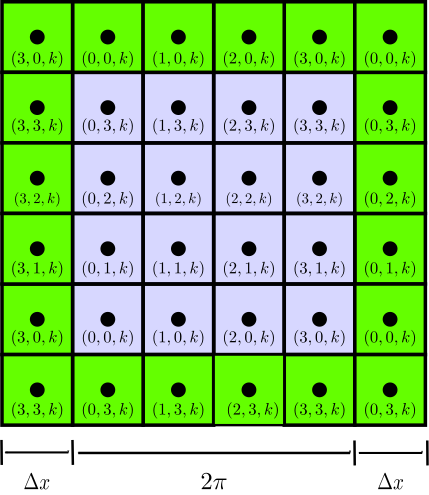
\includegraphics[height=0.35\textheight]{media/rk4/periodic-BCs}
    \caption{Ghost cell examples for $N=4$}
    \label{fig:ghost-cell-example}
\end{figure}

Lastly, after every time step the location of the coordinate point $x$ is
checked to ensure it is still within the domain $0 \leq x_{1}, x_{2}, x_{3}
\leq 2\pi$. Again since the ALES code is periodic, the location of the
coordinate point can be easily adjusted by either adding $2\pi$ for cases
where $x<0$ or subtracting $2\pi$ for cases where $x>0$, namely
\begin{equation}
    x = 
    \begin{cases}
        x           \text{\hspace{1.3cm}if $ 0 \leq x \leq 2\pi$}  \\
        x + 2\pi    \text{\hspace{0.3cm}if $ x < 0$}  \\
        x - 2\pi    \text{\hspace{0.3cm}if $ x > 2\pi$}     \\
    \end{cases}
\end{equation}
An two-dimensional example of how the location of $x$ is adjusted in the
forwards and backwards tracking code can be seen in
Fig~(\ref{fig:location-adjustment}), where we can see how the initial point
in red being relocated to other side of the domain.
\begin{figure}[H]
    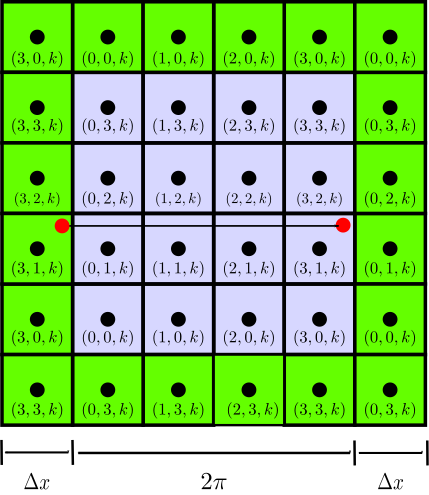
\includegraphics[height=0.35\textheight]{media/rk4/location-adjustment}
    \caption{Example of how the $x$ location is adjusted using periodic B.C.s}
    \label{fig:location-adjustment}
\end{figure}


        

\subsection{Comparison}
